\documentclass[a4paper]{article}
\usepackage{graphicx}
\usepackage[utf8]{inputenc}
\usepackage[english, serbian]{babel}

\title{UseCase: Prijavljivanje korisnika}
\date{10.11.2018.}
\author{Božidar}

\begin{document}

\maketitle

\begin{itemize}
    \item Naziv: Prijavljivanje korisnika
    \item Akter: Korisnik sistema (Administrator, Glavni urednik, Urednik, Recenzent, Autor)
    \item Kratak opis: Korisnik unosi potrebne podatke kako bi se ulogovao u sistem
    \item Osnovni tok događaja:(ponavljati korak 2 željeni broj puta)
        \begin{enumerate}
            \item Korisnik unosi svoju email adresu i sifru u polja koja su za to predoredjena
            \item Pokusava da se prijavi na sistem
            \item Nakon uspesnoj autentikaciji korisnika prikazuje mu početna stranica u zavisnosti od uloge:
            \begin{enumerate}
                \item Administrator - admin panel za upravljanje sistemom
                \item Glavni urednik - lista novopristiglih radova
                \item Urednik - lista radova koji su poslednji dodeljeni od strane glavnog urednika
                \item Recenzent - lista radova koji su poslednji ponudjeni za recenziju od strane urednika
                \item Autor - listu svojih radova
            \end{enumerate}
        \end{enumerate}
    \item Alternativni tok događaja:
        \begin{enumerate}
            \item Autentikacija korisnika nije uspela
                \begin{enumerate}
                    \item Nakon 2. koraka sistem ispisuje poruku o neuspešnoj autentikaciji.
                    \item Korisnik ponavlja korake 1. i 2.
                \end{enumerate}
        \end{enumerate}
\end{itemize}

\begin{figure}
    \centering
    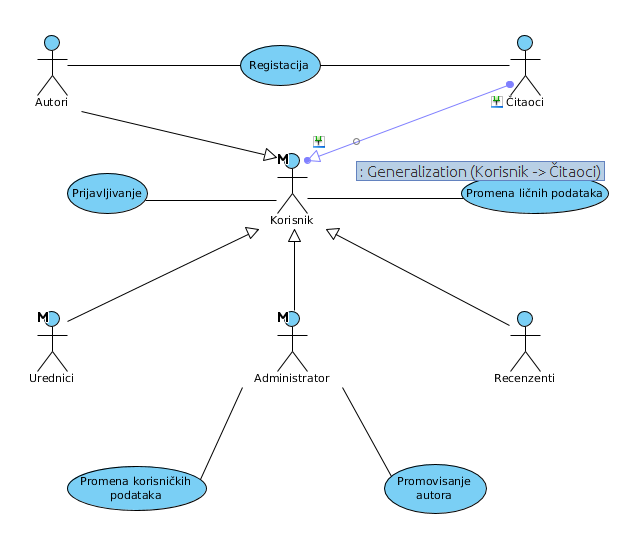
\includegraphics[width=\linewidth]{usecasePrijavljivanje.png}
    \caption{UseCase screenshot}
    \label{fig:my_label}
\end{figure}


\end{document}
